\documentclass{article}
\usepackage{hyperref}
\usepackage{listings}
\usepackage{color}
\usepackage{xcolor}
\usepackage{geometry}
\usepackage{graphicx}
\usepackage{amsmath}
\usepackage{caption}
\usepackage{subcaption}
\geometry{margin=1in}
\pdfminorversion=6

\newcommand\TODO[1]{\textcolor{red}{TODO: #1}}

\newcommand\header[2]{
    \begin{center}
        {\large
        UCSD CSE 168 Assignment #1: \\
        \vspace{0.3cm}
        \Large
        #2}
    \end{center}
}

\definecolor{dkgreen}{rgb}{0,0.6,0}
\definecolor{gray}{rgb}{0.5,0.5,0.5}
\definecolor{mauve}{rgb}{0.58,0,0.82}
\lstset{frame=tb,
        aboveskip=3mm,
        belowskip=3mm,
        showstringspaces=false,
        columns=flexible,
        basicstyle={\small\ttfamily},
        numbers=none,
        numberstyle=\tiny\color{gray},
        keywordstyle=\color{blue},
        commentstyle=\color{dkgreen},
        stringstyle=\color{mauve},
        breaklines=true,
        breakatwhitespace=true,
        tabsize=2
}

\hypersetup{colorlinks=true}


\begin{document}

\header{1}{Ray Tracing}
\setcounter{section}{-1}

In our first homework, we are going to implement a simple ray tracer (almost) from scratch.
We will provide some utility code such as the vector class and parallel threading. 
However, you will have to implement the rest yourself. Trust me, it will be fun!

Our homeworks are mostly inspired by the book \href{https://raytracing.github.io/}{Ray Tracing in One Weekend (RTOW)} (click the link for free access of the e-book). You are expected to read the relevant chapters of the book before implementing your own version. The structure of the homeworks is also largely inspired by \href{https://cs87-dartmouth.github.io/Fall2022/assignments.html}{CS 87/287 at Dartmouth} designed by Wojciech Jarosz (a UCSD alumni!).

\section{Building Torrey}
We are going to build our code on top of (a currently very barebone) renderer \emph{torrey}. Torrey already includes all the third party libraries (pugixml, pcg, stb\_image, tinyexr, miniz, tinyply) in its repo and all you need to do is to clone the repo and build it using CMake (assuming you are in a Unix-like system):
\begin{lstlisting}[language=bash]
  git clone https://github.com/BachiLi/torrey_public
  mkdir build
  cd build
  cmake ..
  make -j
\end{lstlisting}

After building, you should see an executable \lstinline{torrey}. Try typing the following command:
\begin{lstlisting}[language=bash]
  torrey -hw 1_1
\end{lstlisting}
It will generate an image \lstinline{hw_1_1.exr} that looks like the following:
\begin{figure}[h]
    \centering
    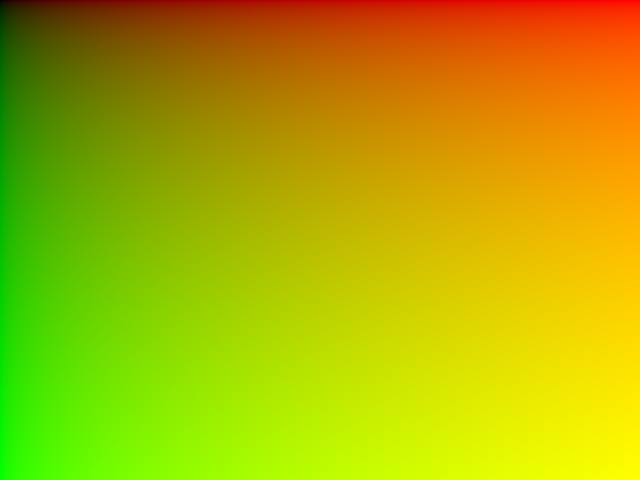
\includegraphics[width=0.5\linewidth]{imgs/hw_1_1_before.png}
    \caption{Image output by the homework 1.1 code before your modification.}
    \label{fig:hw_1_1_before}
\end{figure}

\lstinline{.exr} is an image format that is suitable for storing \emph{high-dynamic range} images. Basically, instead of storing 8-bit (0-255) per color channel, we store a floating point number per channel. To view \lstinline{.exr}, I recommend using \href{https://github.com/wkjarosz/hdrview}{HDRView} or \href{https://github.com/Tom94/tev}{Tev}.

Read \lstinline{main.cpp}, \lstinline{hw1.cpp}, \lstinline{vector.h}, and \lstinline{image.h} to understand the current code structure.

\section{Sending rays from the camera}
To do ray tracing, we need to first shoot rays from the camera. In this first step, we will generate camera rays for all the pixels. The goal of our first task is to visualize the camera ray direction (normalized to unit length per pixel).

First, read \href{https://raytracing.github.io/books/RayTracingInOneWeekend.html#rays,asimplecamera,andbackground}{Chapter 4.2} of the first RTOW book and understand its content.

We will use a very simple perspective camera for now. The position is fixed at $(0, 0, 0)$, and the camera is facing towards $(0, 0, 1)$ with an up vector $(0, 1, 0)$, right vector $(1, 0, 0)$, and focal length of $1$ (note that this is subtly different from RTOW). We will make the camera ``positionable'' later. For each pixel, we will shoot a ray from the center of the pixel (for a pixel $(x, y) \in [0, \text{width}] \times [0, \text{height}]$, we shoot a ray in $(x + 0.5, y + 0.5)$). Your task is to output the \emph{unit length} ray direction per pixel. Some of the pixels will have negative color but that is fine. We provide the \lstinline{.exr} code for your comparison.

\begin{figure}[h]
    \centering
    
\includegraphics[width=0.5\linewidth]{imgs/hw_1_1_after.png}
    \caption{Image output by the homework 1.1 code after your modification.}
    \label{fig:hw_1_1_after}
\end{figure}


%\bibliographystyle{plain}
%\bibliography{refs}

\end{document}
